\chapter{Захворювання печінки}

\section{Які існують захворювання печінки?}

Існує велика кількість патології печінки, яку умовно можна розділити на \textit{дифузну} та вогнищеву. \sidenote[][40pt]{Хвороби печінки та їх лікування вивчає окрема наукова галузь медицини - гепатологія. }

При вогнищевій патології уражується частнина органа. До вогнищевої патології відносяться злоякісні та доброякісні пухлини, абсцеси, кістозна патологія та ін.

При дифузній патології внаслідок хронічного запалення (або дії іншого уражуючого фактору) пошкоджується вся паренхіма (тканина) органу. До дифузної патології відносяться цироз, фіброз, жировий гепатоз, амілоїдоз та ін.

\begin{figure}
  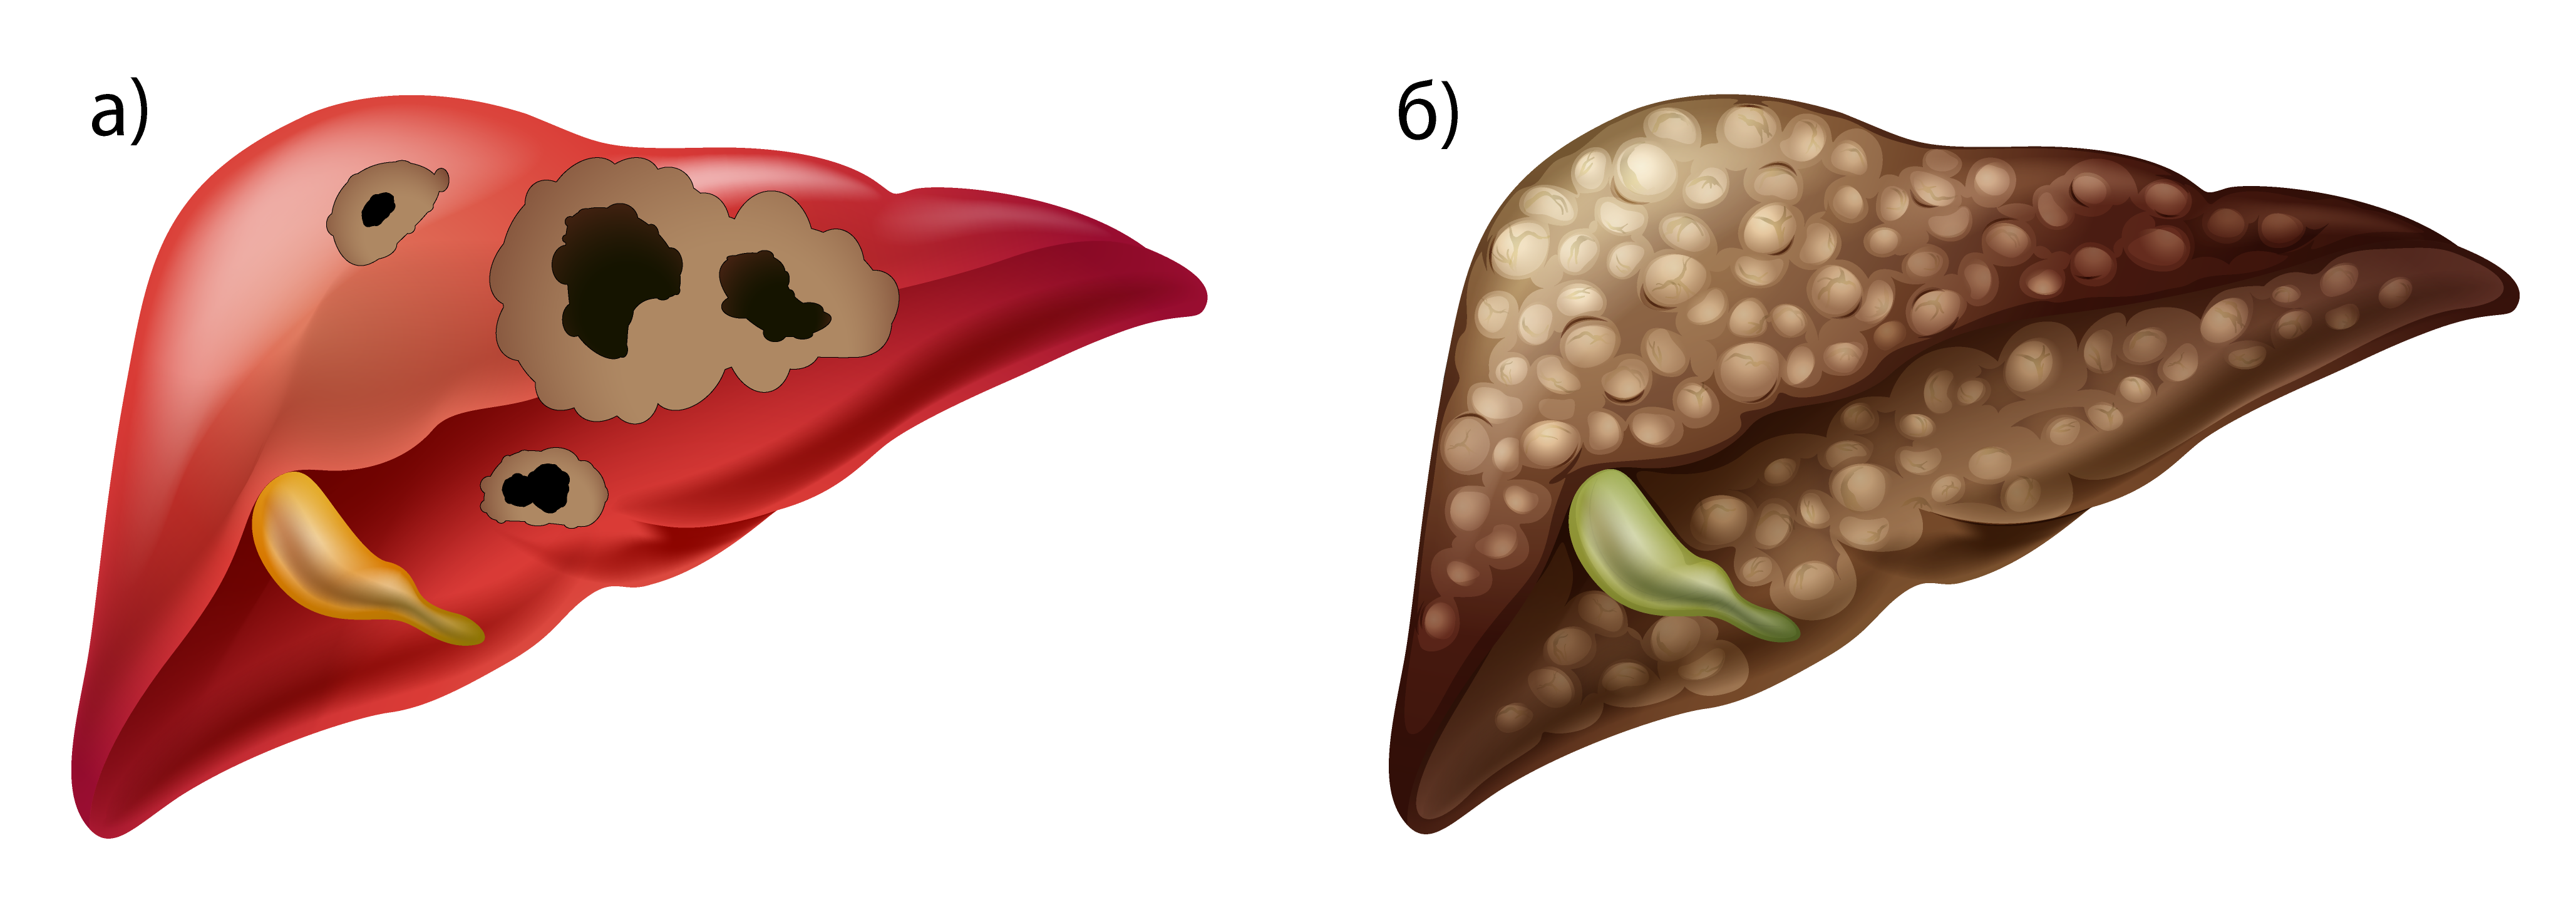
\includegraphics{Figures/Liver diseases_Diffuse and Nodular.png}
%  \checkparity This is an \pageparity\ page.%
  \caption{Патологія печінки. а) вогнищева патологія -- пухлина печінки, б) дифузна патологія -- цироз печінки }
  \label{fig:textfig}
  %\zsavepos{pos:textfig}
\end{figure}

\section{Які є види пухлин печінки?}

Пухлини печінки є основним видом її вогнищевої патології.
Розрізняють злоякісні та доброякісні пухлини печінки.

\begin{marginfigure}[20pt]%
  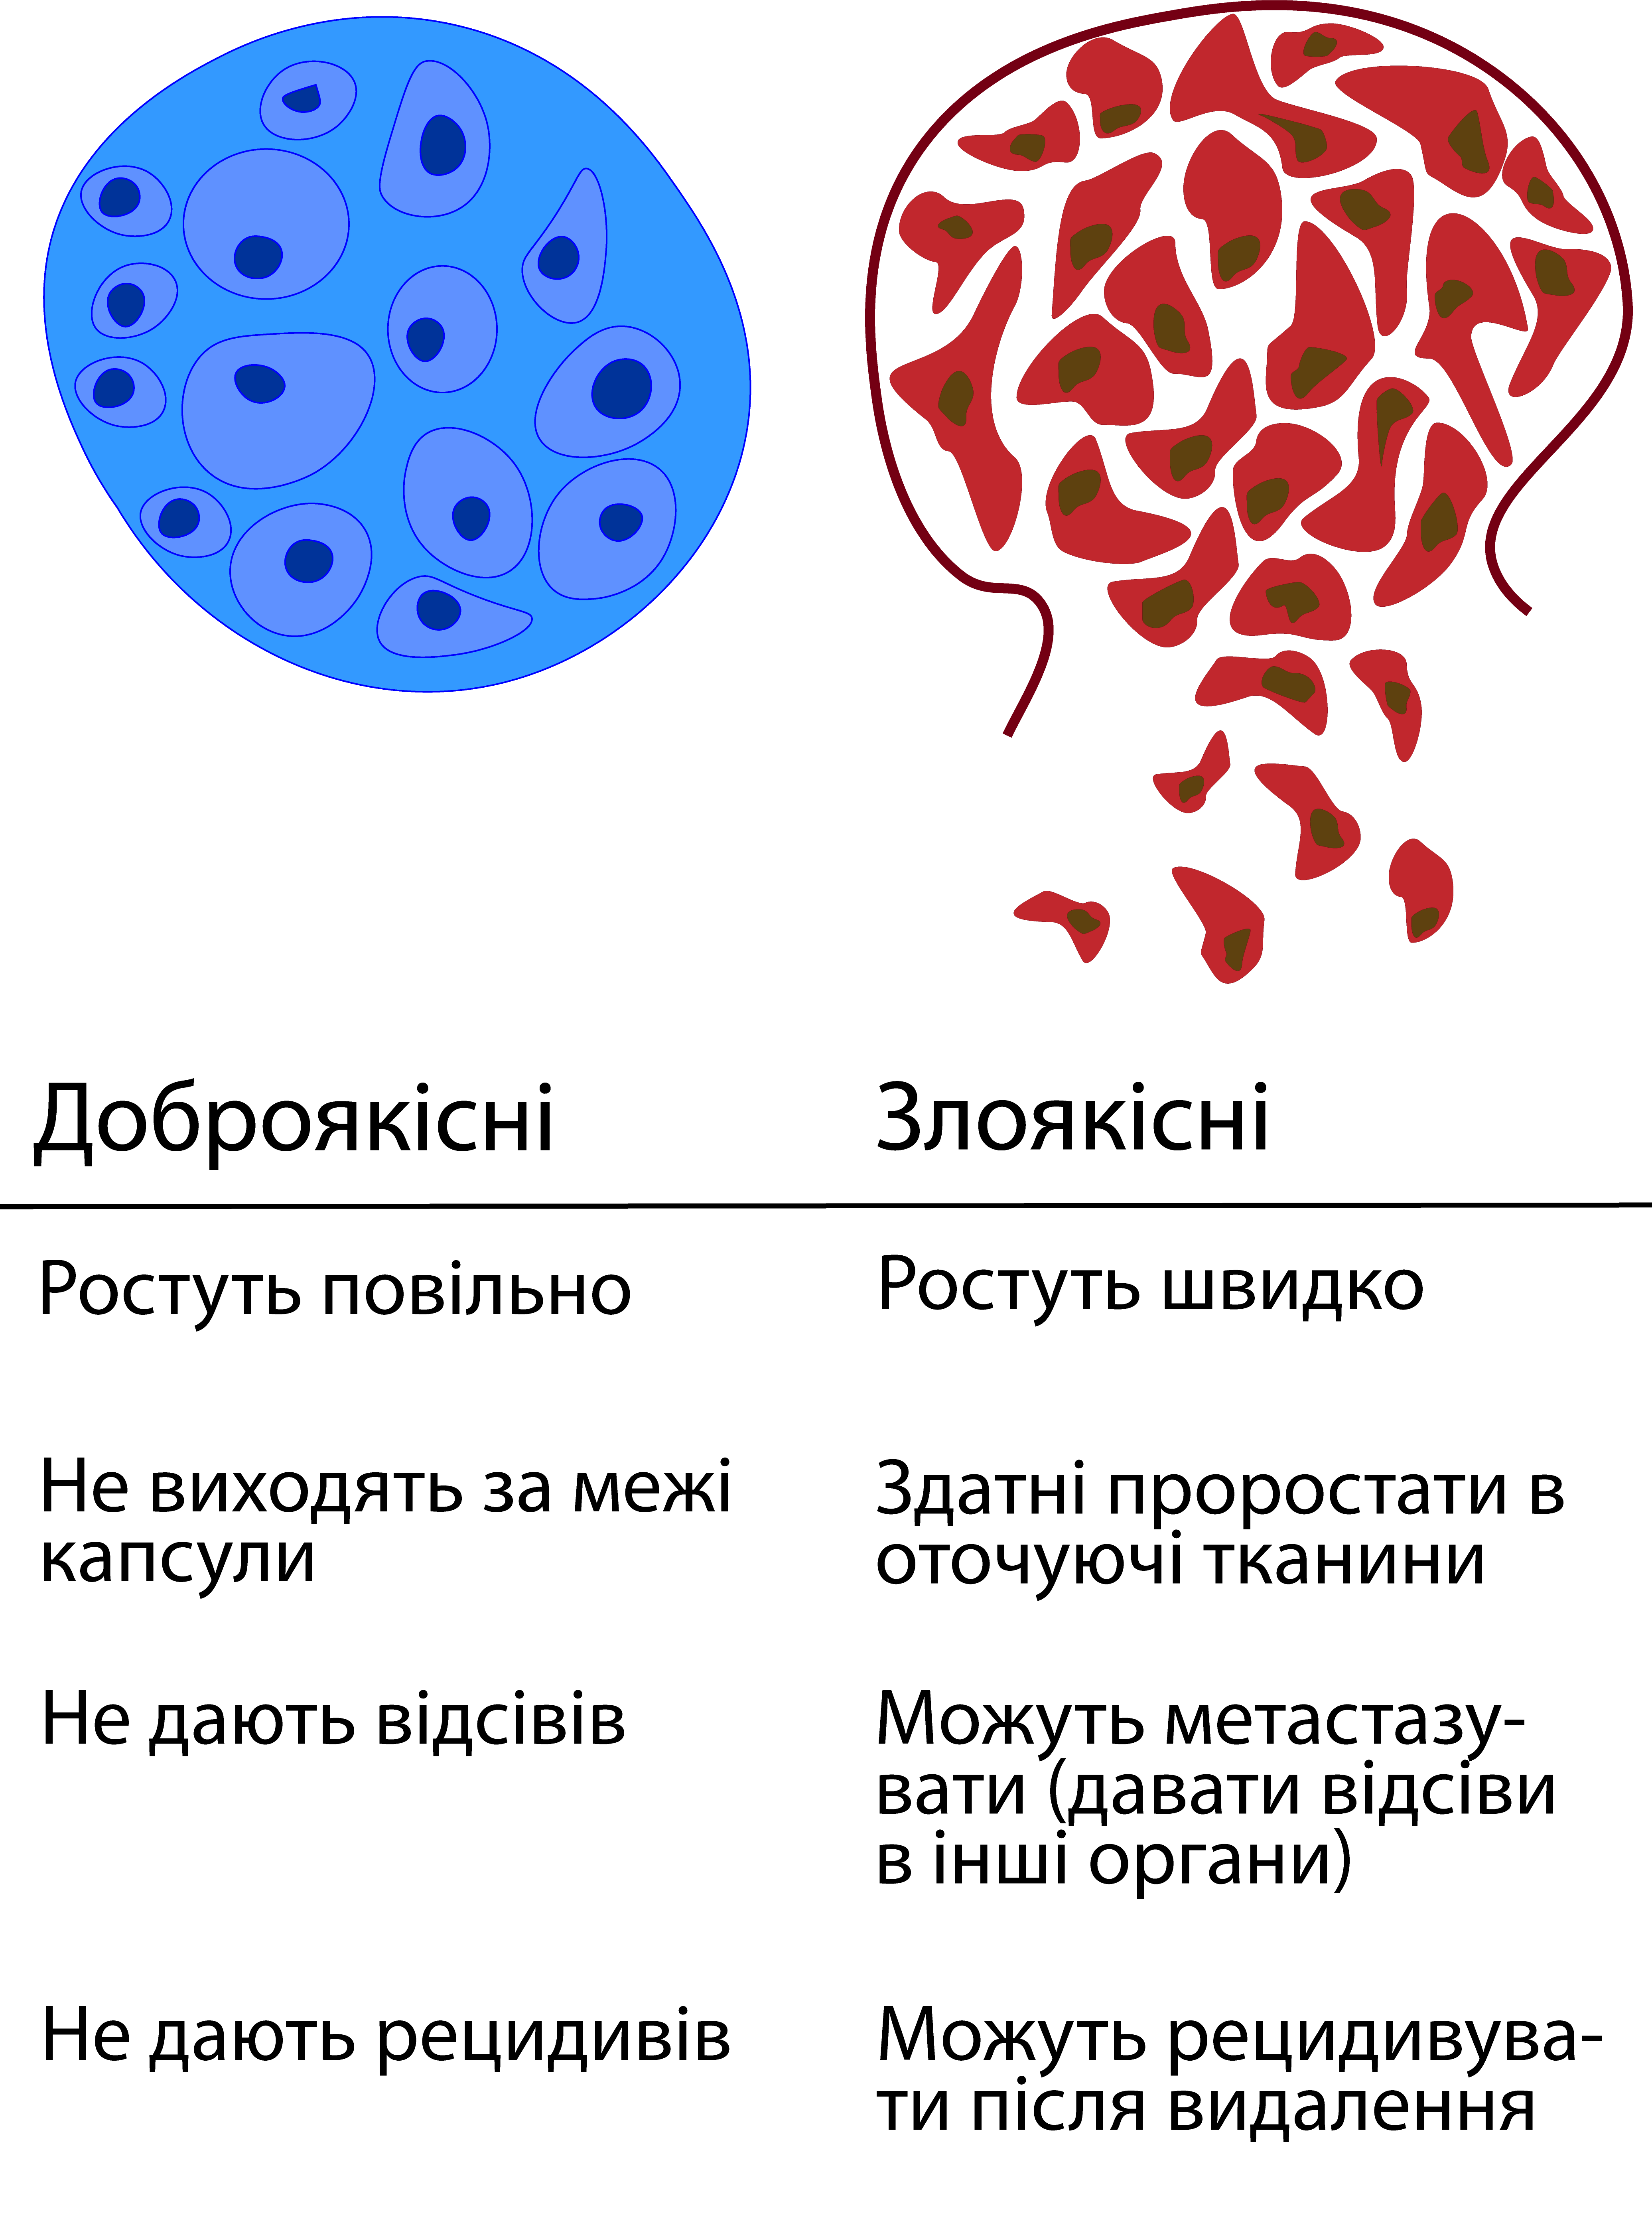
\includegraphics[width=\linewidth]{Figures/Benign vs malignant.png}
  \caption{Відмінності доброякісних та злоякісних пухлин}
  \label{fig:benignvsmalignant}
\end{marginfigure}

\section{Які є види злоякісних новоутвореннь печінки?}

Виділяють: 
\begin{enumerate}
    \item первинні пухлини печінки - ті що беруть своє первинне походження з клітин печінки або жовчних протоків, та
    \item вторинні (або метастатичні) - пухлини, які з’явились в печінці внаслідок міграції злоякісних клітин з інших органів
\end{enumerate} 

До первинних пухлин відносять такі захворювання:

\begin{itemize}
    \item Пухлини, що походять з гепатоцитів, клінтин тканини печінки
        \begin{itemize}
            \item гепатоцелюлярна карцинома (первинний рак печінки)
            \begin{marginfigure}[-10pt]%
                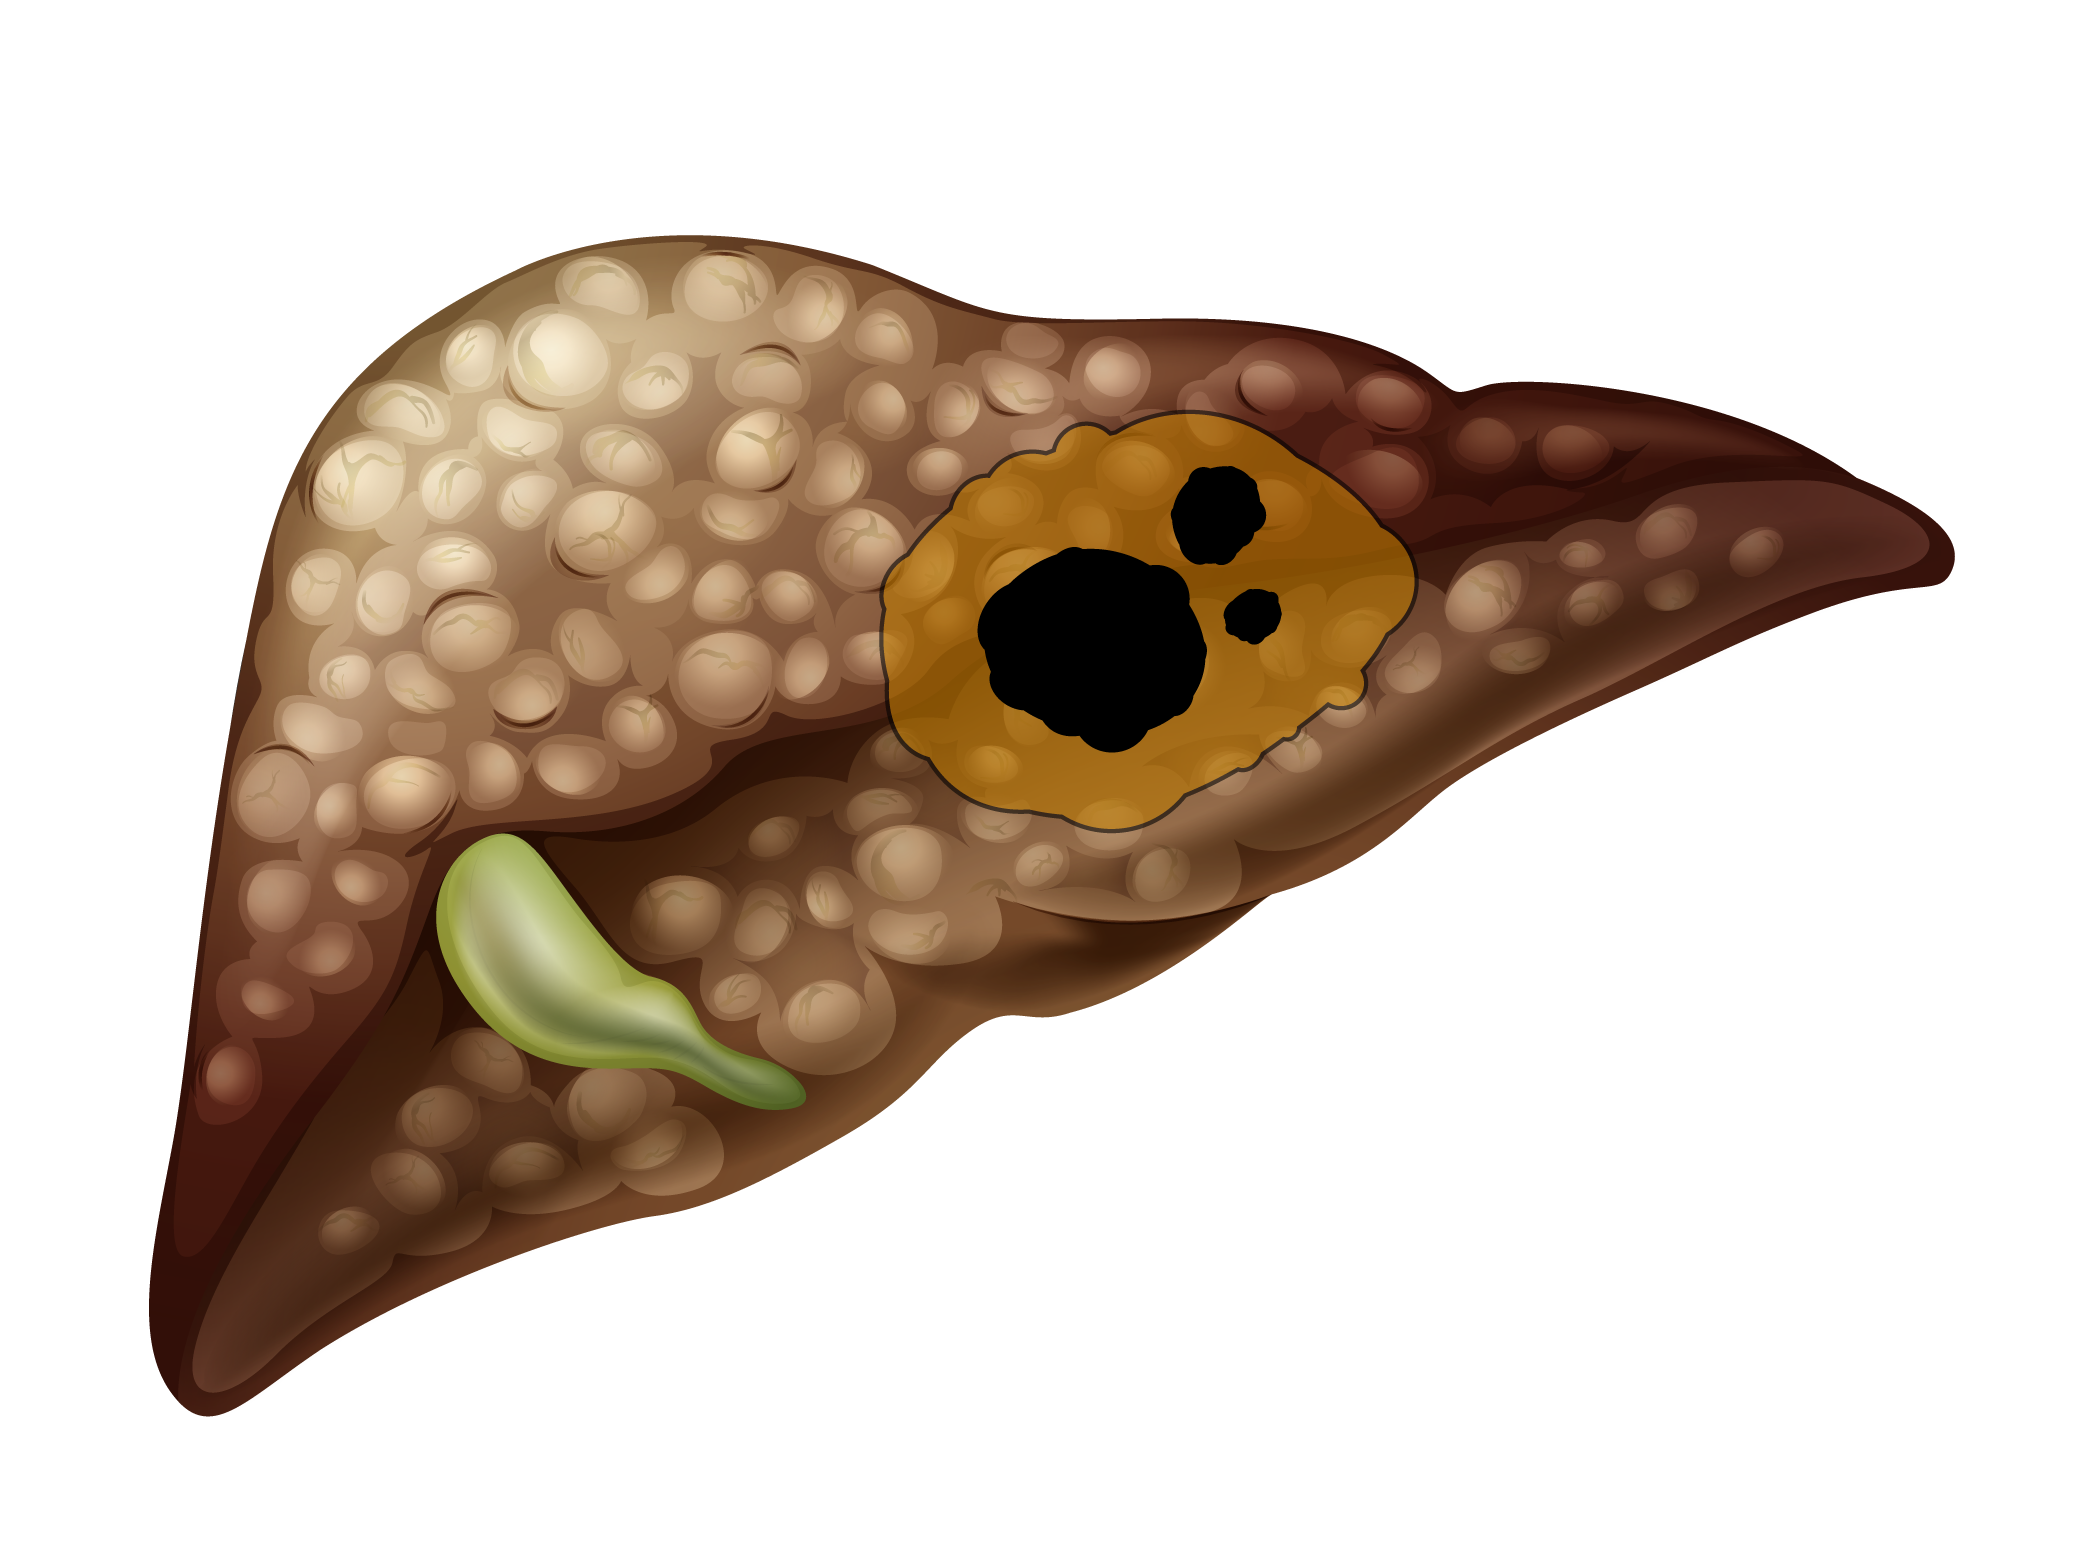
\includegraphics[width=\linewidth]{Figures/HCC.png}
                \caption{Гепацтоцеллюлярна карцинома (ГЦК). Первинний рак печінки -- пухлина, яка найчастіше виникає на фоні цирозу печінки}
                 \label{fig:hcc}
            \end{marginfigure}
            
            \item гепатобластома (особливий тип злоякісної пухлини печінки, що виникає переважно в дитячому віці)
            \item рак біліарного тракту (внутрішньопечінкова холангіокарцинома)
        \end{itemize}
    \item Пухлини, що походять біліарного тракту (жовчних протоків) 
        \begin{itemize}
            \item внутрішньопечінкова холангіокарцинома
            \item хіларна холангіокарцинома (рак розвилки жовчних шляхів або хвороба Клацкіна)
            \begin{marginfigure}[10pt]%
                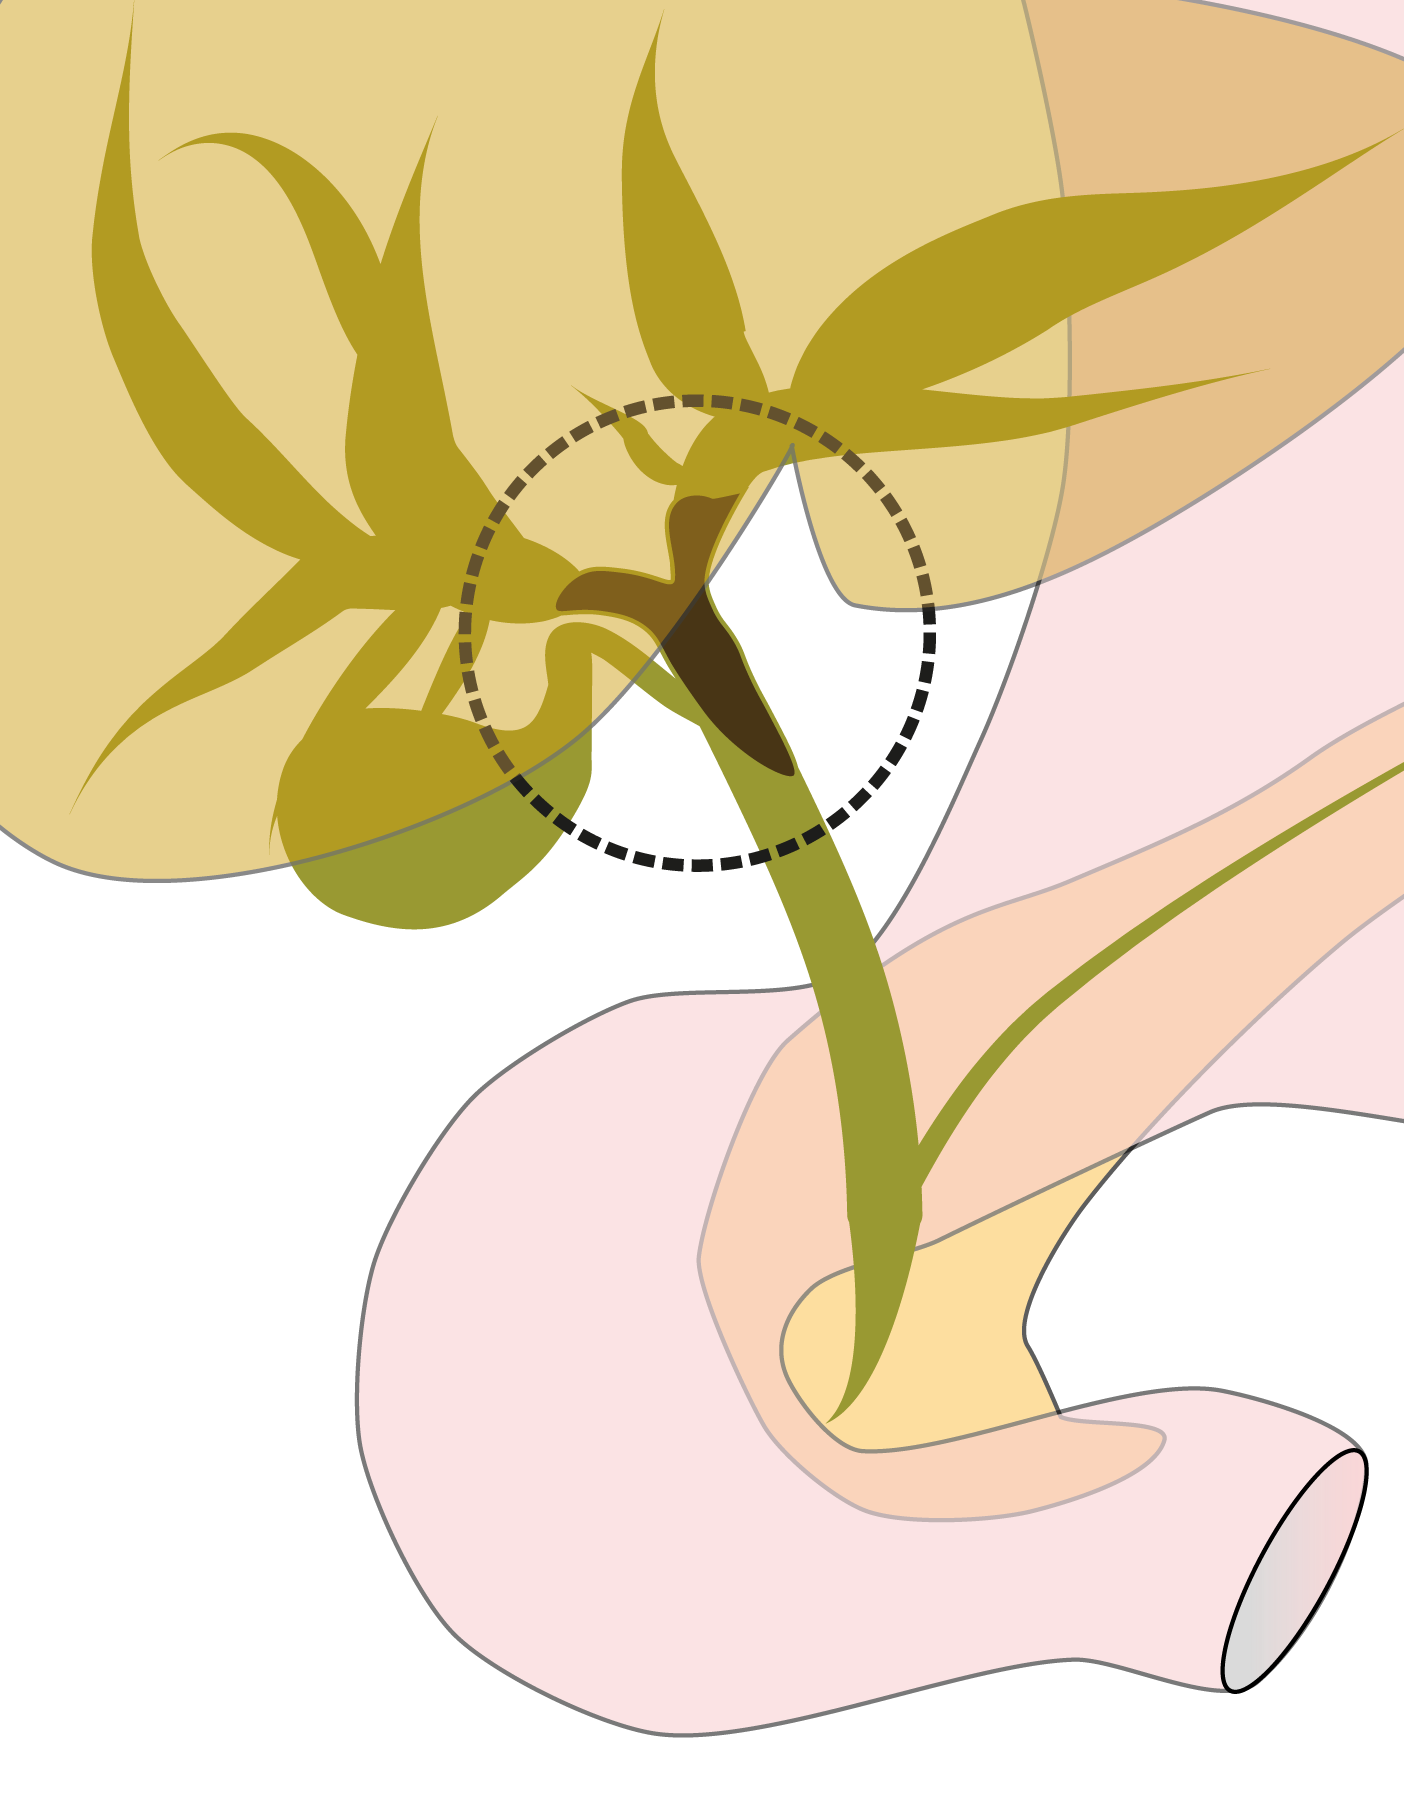
\includegraphics[width=\linewidth]{Figures/PHCC.png}
                \caption{Хіларна холангіокарцинома, або пухлина Клацікіна. Через локалізацію в зоні розвилки жовчних шляхів пухлина перекриває відтік жовчі та призводить до механінчої жовтяниці}
                 \label{fig:phcc}
            \end{marginfigure}
            
            \item рак жовчного міхура
        \end{itemize}
\end{itemize}
	
До вторинних пухлин відносять:
\begin{itemize}
    \item метастази колоректального раку
    \item метастази нейроендокринних пухлин
    \item метастази іншого походження
\end{itemize}

Більшість злоякисних новоутвореннь печінки потребують хірургічного лікування - резекції печінки

\begin{marginfigure}[10pt]%
  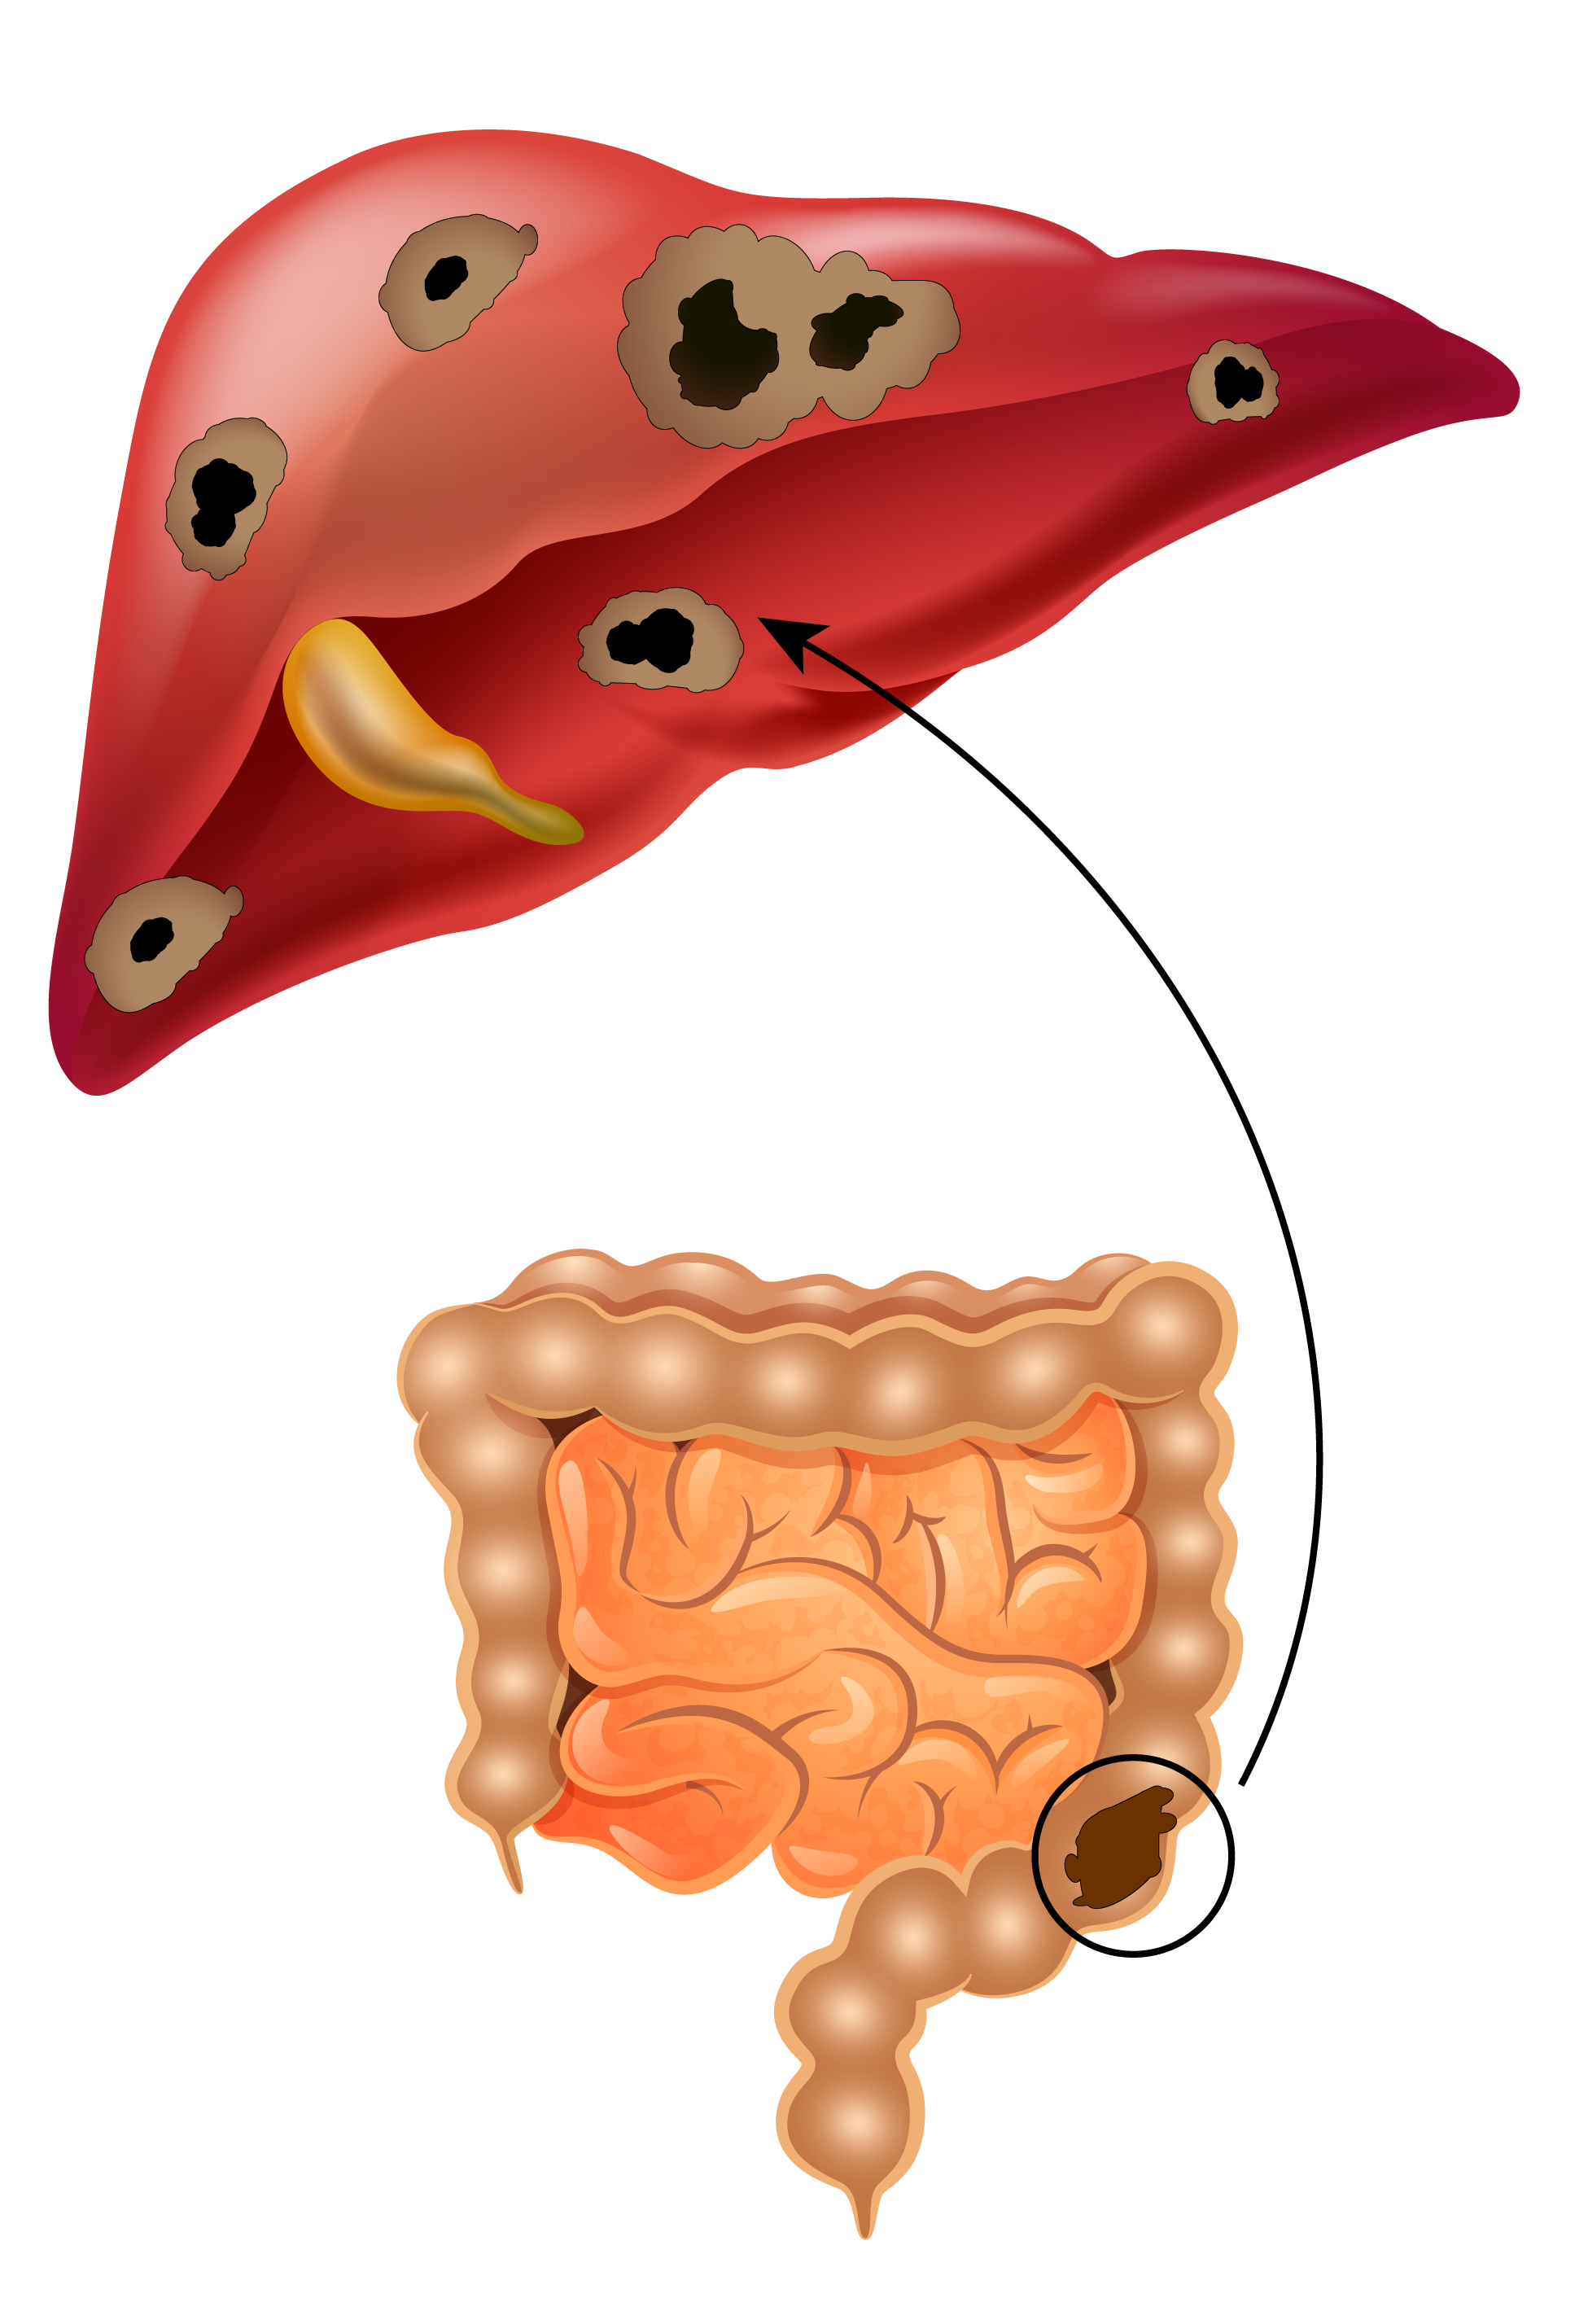
\includegraphics[width=\linewidth]{Figures/CRLM.png}
  \caption{Метастази колоректального раку печінки. Вторинні ураження процес може давати відсіви навіть тоді, коли первинна пухлина видалена}
  \label{fig:crlm}
\end{marginfigure}

\newpage
\section{Які захворювання відносять до доброякісних новоутвореннь печінки?}

До доброякісних новоутвореннь печінки відносять 
\begin{itemize}
    \item гемангіоми
    \item фокальну нодулярну гіперплазію (ФНГ)
    \item аденоми
    \item кісти (прості, ехінококові) та кістозні пухлини печінки (цистаденоми)
\end{itemize}

В більшості випадків при доброякісній патології печінки хірургічне втручання не потрібне. В разі великого симптоматичного ураження або за наявності ризика ускладненнь (розрив, кровотеча, перетворення на злоякісну пухлину) виконують мініінвазивні втручання - пункції кист або абсцесів, лапароскопічні резекції аденом, гемангіом, ФНГ та ін.  


\section{Кому необхідне хірургічне втручання на печінці?}

Хірургічні втручання (\textcolor{red}{резекція}, \textcolor{red}{трансплантація}  або \textcolor{red}{інтервенційне втручання}) на печінці показані пацієнтам, що страждають на вогнищеву або термінальні стадії дифузної патології печінки. 

Рішення про необхідність оперативного втручання після всебічного обстеження приймає виключно мультидисциплінарна коміссія, що обов’язково включає висококваліфікованого фахового спеціаліста - гепатобіліарного хірурга із достатнім клінічним досвідом таких втручаннь. 